%%  Tanque punzado (igual casquete esférico pero elipsoidal) (C)
\item Un tanque sufre, en una de sus paredes verticales planas, una abolladura
como se muestra en la figura \ref{fig:bollo}. La misma puede considerarse
como un cilindro de sección elipsoidal (semiejes  de longitud \textbf{A} y
\textbf{B}) y largo $L$. Calcule cuál es la fuerza hidrostática resultante
sobre la abolladura (en función de sus dimensiones) y qué torque genera
respecto a los puntos de concentración de tensiones (\textbf{a} y \textbf{b}). Exprese el resultado en términos de los parámetros del problema:
\begin{equation*}
\rho \qquad A \qquad B \qquad L \qquad H_0
\end{equation*}

\begin{figure}[h!!!!]
  \centering
  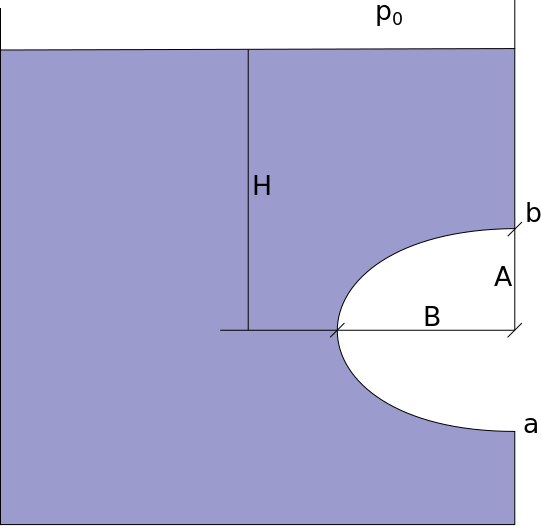
\includegraphics[width=0.4\textwidth]{bollo.png}
  \caption{Abolladura elipsoidal en pared plana}
  \label{fig:bollo}
\end{figure}

